
\documentclass[a4paper,12pt]{scrbook}
\usepackage{amsmath,amssymb,amsthm}
\usepackage{fancyvrb}
\usepackage{parskip}
\usepackage{lastpage}
\usepackage{verbatim,boxedminipage,enumitem}
\usepackage{ifthen}
\usepackage{color,graphicx}
\usepackage{pgf}
\usepackage{longtable}
\usepackage{upquote}
%\usepackage[all]{xy}
\usepackage{tobiShell}
\usepackage{tikz}
\usetikzlibrary{automata}
\usetikzlibrary{arrows}
\usepackage{pgf,pgfarrows,pgfnodes}
\usepackage{pgfplots}
\usepackage{circuitikz}
\usetikzlibrary{circuits}
\usetikzlibrary{circuits.logic.US}
\usepackage{mymath}
\usepackage{python}
%------------------------------------------------------------------
% Verbatim for console window - single line frame, no line numbers
%------------------------------------------------------------------
\DefineVerbatimEnvironment%
 {console}{Verbatim}
 {frame=single}

%--------------------------------------------------------
% Remove the vertical spacing before and after Verbatim.
%--------------------------------------------------------
\usepackage{atbeginend}
\BeforeBegin{console}{\mbox{}\\ \begin{minipage}{\textwidth}\vspace{3pt}}
\AfterEnd{console}{\vspace{4pt} \end{minipage} \\ }

\begin{document}
\thispagestyle{empty}

\begin{center}
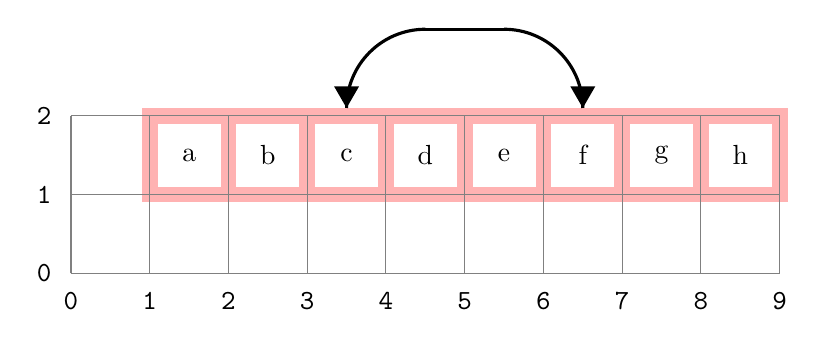
\begin{tikzpicture}

\draw (1.5, 1.5)
  node[draw, line width=0.2cm, , color=red!30!white,
       rounded corners=0cm, inner sep=0cm] {

\begin{minipage}[t][1.0cm]{1.0cm}
\mbox{}

\end{minipage}

};\draw (1.5, 1.5) node[color=black] {a};
\draw (2.5, 1.5)
  node[draw, line width=0.2cm, , color=red!30!white,
       rounded corners=0cm, inner sep=0cm] {

\begin{minipage}[t][1.0cm]{1.0cm}
\mbox{}

\end{minipage}

};\draw (2.5, 1.5) node[color=black] {b};
\draw (3.5, 1.5)
  node[draw, line width=0.2cm, , color=red!30!white,
       rounded corners=0cm, inner sep=0cm] {

\begin{minipage}[t][1.0cm]{1.0cm}
\mbox{}

\end{minipage}

};\draw (3.5, 1.5) node[color=black] {c};
\draw (4.5, 1.5)
  node[draw, line width=0.2cm, , color=red!30!white,
       rounded corners=0cm, inner sep=0cm] {

\begin{minipage}[t][1.0cm]{1.0cm}
\mbox{}

\end{minipage}

};\draw (4.5, 1.5) node[color=black] {d};
\draw (5.5, 1.5)
  node[draw, line width=0.2cm, , color=red!30!white,
       rounded corners=0cm, inner sep=0cm] {

\begin{minipage}[t][1.0cm]{1.0cm}
\mbox{}

\end{minipage}

};\draw (5.5, 1.5) node[color=black] {e};
\draw (6.5, 1.5)
  node[draw, line width=0.2cm, , color=red!30!white,
       rounded corners=0cm, inner sep=0cm] {

\begin{minipage}[t][1.0cm]{1.0cm}
\mbox{}

\end{minipage}

};\draw (6.5, 1.5) node[color=black] {f};
\draw (7.5, 1.5)
  node[draw, line width=0.2cm, , color=red!30!white,
       rounded corners=0cm, inner sep=0cm] {

\begin{minipage}[t][1.0cm]{1.0cm}
\mbox{}

\end{minipage}

};\draw (7.5, 1.5) node[color=black] {g};
\draw (8.5, 1.5)
  node[draw, line width=0.2cm, , color=red!30!white,
       rounded corners=0cm, inner sep=0cm] {

\begin{minipage}[t][1.0cm]{1.0cm}
\mbox{}

\end{minipage}

};\draw (8.5, 1.5) node[color=black] {h};\draw[line width=0.04cm,black,->,>=triangle 60] (3.5,2.1001) -- (3.5,2.1);
\draw[line width=0.04cm,black,->,>=triangle 60] (6.5,2.1001) -- (6.5,2.1);
\draw[line width=0.04cm,black] (4.5,3.1) -- (5.5,3.1);
\draw[line width=0.04cm,black] (6.5,2.1001) arc (0:90:1);\draw[line width=0.04cm,black] (3.5,2.1001) arc (180:90:1);\draw[gray] (0.0,0.0) -- (0.0,2);
\draw[gray] (1.0,0.0) -- (1.0,2);
\draw[gray] (2.0,0.0) -- (2.0,2);
\draw[gray] (3.0,0.0) -- (3.0,2);
\draw[gray] (4.0,0.0) -- (4.0,2);
\draw[gray] (5.0,0.0) -- (5.0,2);
\draw[gray] (6.0,0.0) -- (6.0,2);
\draw[gray] (7.0,0.0) -- (7.0,2);
\draw[gray] (8.0,0.0) -- (8.0,2);
\draw[gray] (9.0,0.0) -- (9.0,2);
\draw[gray] (0.0,0.0) -- (9,0.0);
\draw[gray] (0.0,1.0) -- (9,1.0);
\draw[gray] (0.0,2.0) -- (9,2.0);
\draw(0, 0) node [font=\ttfamily, label=below:{\texttt{0}}] {};
\draw(1, 0) node [font=\ttfamily, label=below:{\texttt{1}}] {};
\draw(2, 0) node [font=\ttfamily, label=below:{\texttt{2}}] {};
\draw(3, 0) node [font=\ttfamily, label=below:{\texttt{3}}] {};
\draw(4, 0) node [font=\ttfamily, label=below:{\texttt{4}}] {};
\draw(5, 0) node [font=\ttfamily, label=below:{\texttt{5}}] {};
\draw(6, 0) node [font=\ttfamily, label=below:{\texttt{6}}] {};
\draw(7, 0) node [font=\ttfamily, label=below:{\texttt{7}}] {};
\draw(8, 0) node [font=\ttfamily, label=below:{\texttt{8}}] {};
\draw(9, 0) node [font=\ttfamily, label=below:{\texttt{9}}] {};
\draw(0, 0) node [font=\ttfamily, label=left:{\texttt{0}}] {};
\draw(0, 1) node [font=\ttfamily, label=left:{\texttt{1}}] {};
\draw(0, 2) node [font=\ttfamily, label=left:{\texttt{2}}] {};
\end{tikzpicture}

\end{center}

\end{document}
